\documentclass[12pt,a4paper]{article}

% Paquetes básicos
\usepackage[utf8]{inputenc}
\usepackage[spanish]{babel}
\usepackage{graphicx}
\usepackage{xcolor}
\usepackage{amsmath}
\usepackage{amssymb}
\usepackage{hyperref}
\usepackage{geometry}
\usepackage{listings}
\usepackage{xcolor}
\usepackage{float}
\usepackage{epigraph}
\usepackage{cite}
\usepackage{tcolorbox}
\tcbuselibrary{listings, skins, breakable}
\usepackage{listings}
\usepackage{xcolor}
\usepackage{subcaption}

% Configurar márgenes
\geometry{
    top=2.5cm,
    bottom=2.5cm,
    left=3cm,
    right=3cm
}

% Configurar listings
\lstset{
    basicstyle=\small\ttfamily,
    breaklines=true,
    frame=single,
    numbers=left,
    numberstyle=\tiny,
    captionpos=b
}

% Información del documento
\title{Entrega Final \\
\large - APAAD - }
\author{Marcelo Ferreiro Sánchez\\ Pablo Chantada Saborido \\ Gillermo García Engelmo \\Pepe Romero Conde}
\date{\today}



%% SQL

\definecolor{azulito}{RGB}{186,200,211}
\definecolor{azul_oscuro}{RGB}{35,68,93}

%% SQL listing style
%\lstdefinestyle{SQL}{
%  language=SQL,
%  basicstyle=\ttfamily\small,
%  keywordstyle=\color{sqlblue}\bfseries,
%  commentstyle=\color{sqlgreen},
%  stringstyle=\color{orange!60!black},
%  backgroundcolor=\color{sqllight},
%  showstringspaces=false,
%  breaklines=true,
%  frame=none
%}

% Define the tcolorbox for SQL
\newtcolorbox{sqlbox}[1][]{%
  enhanced,
  breakable,
  colback=azulito,
  colframe=azul_oscuro,
  fonttitle=\bfseries,
  fontupper=\ttfamily,
%  title=SQL Code,
%  listing only,
%  listing options={style=SQL},
  #1
}

%%


\begin{document}

\maketitle

\tableofcontents

\newpage

\section{Introdución}

\section{Diseño del modelo lógico e implementación del DW en Oracle}

\subsection{Rediseño do modelo da práctica anterior}

\textcolor{red}{
\begin{itemize}
	\item Proponer el diagrama del modelo lógico para el diseño realizado (normalmente será un modelo
sencillo, en estrella o en copo de nieve), incluyendo una breve explicación de las decisiones tomadas
y crear las tablas resultantes en Oracle.
	\item Crear las tablas necesarias en Oracle.
\end{itemize}}

Despóis da corrección da entrega anterior modificamos o DFM do seguinte xeito:
\begin{itemize}
	\item Baixamos as dimensións de \texttt{Hospedador} e \texttt{Lugar} ó nivel de \texttt{Hospedaxe} para evitar o modelo \emph{Copo de neve}, o cal atopamos vantaxoso por gañar simpleza do modelo e velocidade das consultas \cite{evitarSnowflake}.  
	\item Actualizamos o DFM cos atributos da dimensión \texttt{Eventos} especificados no informe.
	\item Cambios sobre o resto de atributos para buscala coherencia co informe anterior.
\end{itemize}


\begin{figure}[h!]
    \centering

    \begin{subfigure}[l]{0.8\textwidth}
        \centering
        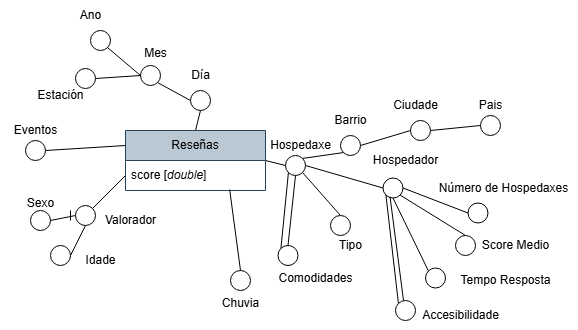
\includegraphics[width=\textwidth]{../../entrega_01/memoria/diagramas/multidimensional.drawio.png}
        \caption{DFM Orixinal}
        \label{fig:dfm-orixinal}
    \end{subfigure}
    \hfill

    \begin{subfigure}[r]{0.8\textwidth}
        \centering
	
\includegraphics[width=\textwidth]{./diagramas/multidimensional.drawio.png}
        \caption{DFM Modificado}
        \label{fig:dfm-modificado}
    \end{subfigure}

  \caption{Diagrama do Modelo de Feitos Dimensional (\emph{DFM})}
  \label{fig:dfm}
\end{figure}




Con todo resulta un modelo en estrela. Donde:
\begin{itemize}
	\item A dimensión \texttt{Chuvia} é dexenerada pois a única métrica que aporta son os mm de precipitacion. Polo tanto ben a podemos incluir na táboa de feitos.
	\item A dimensión \texttt{Hospedaxe} ten dos atributos multievaluados (\texttt{Comodidades} e \texttt{Accesibilidade}, que describen prestacións do aloxsmento e formas de chegar a él, respectivamente) e modelarasen con Táboas Ponte.
	\item A dimensión \texttt{Tempo} está denormalizada, para que en vez de estar representada de forma xerárquica, sea tipo Estrela.
\end{itemize}

\subsection{Creación das Táboas}

\begin{sqlbox}[title={Táboas de dimensión}]
CREATE TABLE dim\_tempo (\\
    tempo\_id INT PRIMARY KEY,\\
    data DATE NOT NULL UNIQUE,\\
    dia INT NOT NULL,\\
    mes INT NOT NULL,\\
    ano INT NOT NULL,\\
    estacion VARCHAR(10) NOT NULL,\\
    tempada\_alta BOOLEAN NOT NULL\\
);\\

CREATE TABLE dim\_lugar (\\
    lugar\_id INT PRIMARY KEY AUTO\_INCREMENT,\\
    barrio\_nome VARCHAR(100) NOT NULL,\\
    cidade\_nome VARCHAR(100) NOT NULL,\\
    pais\_nome VARCHAR(100) NOT NULL,\\
    UNIQUE KEY uk\_place (neighborhood\_name, city\_name, country\_name)\\
);\\

CREATE TABLE dim\_hospedaxe (\\
    hospedaxe\_id INT PRIMARY KEY, -- Xa a tiñamos\\
    precio\_noite DECIMAL(10,2) NOT NULL,\\
    tipo VARCHAR(50) NOT NULL\\
);
\end{sqlbox}

\begin{sqlbox}[title={Táboas ponte}]
CREATE TABLE dim\_comodidades (\\
    comodidade\_id INT PRIMARY KEY AUTO\_INCREMENT,\\
    comodidade\_nome VARCHAR(100) NOT NULL UNIQUE\\
);\\

CREATE TABLE ponte\_hospedaxe\_commodidade (\\
    hospedaxe\_id INT NOT NULL,\\
    commodidade\_id INT NOT NULL,\\
    PRIMARY KEY (hospedaxe\_id, comodidade\_id),\\
    FOREIGN KEY (hospedaxe\_id) REFERENCES dim\_hospedaxe(hospedaxe\_id),\\
    FOREIGN KEY (commodidade\_id) REFERENCES dim\_comodidade(commodidade\_id)\\
);\\

CREATE TABLE dim\_accesibilidade (\\
    accesibilidade\_id INT PRIMARY KEY AUTO\_INCREMENT,\\
    accesibilidade\_nome VARCHAR(100) NOT NULL UNIQUE\\
);\\

CREATE TABLE ponte\_apartment\_accessibility (\\
    apartment\_id INT NOT NULL,\\
    accessibility\_id INT NOT NULL,\\
    PRIMARY KEY (hospedaxe\_id, accesibilidade\_id),\\
    FOREIGN KEY (hospedaxe\_id) REFERENCES dim\_hospedaxe(hospedaxe\_id),\\
    FOREIGN KEY (accesibilidade\_id) REFERENCES dim\_accesibilidade(accesibilidade\_id)\\
);\\
\end{sqlbox}


Notas sobre a implementación:
\begin{itemize}
	\item Na dimensión \texttt{Lugar} usouse \texttt{UNIQUE KEY} para evitar duplicados.
\end{itemize}

\section{Diseño e implementación del ETL}
\textcolor{red}{
\begin{itemize}
\item Diseñar e implementar el proceso ETL (Extract, Transform, Load) completo en Apache Hop, que
permita extraer, depurar/limpiar, transformar y cargar los datos reales de Airbnb en el Data
Warehouse creado en la tarea 2. El proceso deberá automatizar la carga desde los ficheros fuente
hasta las tablas destino en Oracle, garantizando la calidad, consistencia y trazabilidad de los datos.
\item Deberán especificarse los datasets de origen utilizados y documentar las principales
transformaciones realizadas (limpieza, conversión de tipos, homogeneización de categorías,
generación de claves sustitutas, etc.). Además, es necesario describir cómo se tratan valores nulos o
inconsistentes, claves foráneas faltantes, formatos de fecha y moneda, posibles duplicados...
\item El fichero principal de ejecución debe llamarse: \texttt{etl\_airbnb\_main.hpl} y debe ser ejecutable en Hop sin
necesidad de editar las rutas internas. El entregable final debe incluir una carpeta datasets (o enlace
a los ficheros fuente utilizados).
\item El proyecto de Hop debe incluir al menos: Un job principal (.hpl) que coordine la ejecución completa
del proceso ETL con varias transformaciones específicas para cada tabla. El pipeline debe ser
ejecutable de forma completa desde un único job principal.
\item Todas las rutas de ficheros y conexiones deben configurarse de manera relativa (no absolutas) para
facilitar su ejecución en otro entorno. La conexión a Oracle debe configurarse mediante variables de
entorno de Hop (\texttt{\${ORACLE\_HOST}}, \texttt{\${ORACLE\_USER}}, etc.), documentadas en el informe.
\item Todas las transformaciones deben estar claramente nombradas y documentadas dentro del
proyecto Hop. También deben utilizarse Hop variables para parametrizar rutas, nombres de archivos
y credenciales, facilitando la reutilización.
\item No es requisito mínimo, pero se valorará positivamente la inclusión de al menos una de las
siguientes funcionalidades avanzadas: Gestión de dimensiones lentamente cambiantes (SCD tipo 1 o
2), control de carga incremental (detección de nuevos registros o cambios) o mecanismo de logging
o control de errores mediante variables o salidas de Hop.}
\end{itemize}}
\section{Explotación del DW}

\textcolor{red}{
\begin{itemize}
\item Se deben plantear y resolver tres consultas analíticas relevantes sobre el DW implementado. Para
cada consulta, debe incluirse una breve descripción de la consulta (qué hace, y por qué es relevante
o para qué podría aplicarse), y la sentencia SQL que resuelve dicha consulta sobre el esquema
seleccionado. Las consultas deben de ser realistas y diferentes (utilizando diferentes tipos de
consultas analíticas).
\item Se debe crear un informe en Power BI que muestre visualizaciones interactivas de los datos,
incluyendo alguna métrica DAX.
\end{itemize}}

\subsection{Consulta 1: \{nombre\}}

\begin{sqlbox}[title={Consulta 1}]
SELECT name, salary\\
FROM employees\\
WHERE department = `Engineering'\\
ORDER BY salary DESC;
\end{sqlbox}

\subsection{Consulta 2: \{nombre\}}
\subsection{Consulta 3: \{nombre\}}

\newpage

\bibliographystyle{plain}
\bibliography{referencias}


\end{document}
